% useful command to build & clean-up : 
% latexmk -pdf -outdir="French/Portfolio/PDF" -c "French/Portfolio/dossier_competences.tex"
% latexmk -pdf -outdir="French/Portfolio/PDF" "French/Portfolio/dossier_competences.tex"
% latexmk -c "French/Portfolio/dossier_competences.tex"
% find French/Portfolio/PDF -type f \( -name "*.aux" -o -name "*.log"  \) -delete


\documentclass{article}
\usepackage[scaled]{helvet}

\usepackage{textcomp} % for \textquotesingle
\renewcommand{\familydefault}{\sfdefault} % applies font
\usepackage{tcolorbox}
\usepackage{xcolor}
\usepackage{amssymb}
\usepackage[left=0.1in, right=0.1in, top=0.55in, bottom=0.55in]{geometry}
\usepackage{graphicx}
\usepackage{tikz}

\usepackage{hyperref}
\usepackage{enumitem}
\usepackage{fancyhdr}
\usepackage{titlesec}
\usepackage{microtype}
\usepackage{colortbl}
\usepackage{array} % Required for m{...} column type
\usepackage{lastpage} % Required for \pageref{LastPage} to get the total number of pages




% Page style setup

\definecolor{titleBlue}{RGB}{0, 102, 204}
\definecolor{skyblue}{RGB}{135,206,235}
\definecolor{deepBlue}{RGB}{80,100,255} 
\definecolor{mainBlue}{RGB}{0, 51, 102} 
\definecolor{secondaryBlue}{RGB}{0, 153, 204} %
\definecolor{steelBlue}{RGB}{70, 130, 180}
\definecolor{darkCyan}{RGB}{0, 139, 139}
\definecolor{cream}{RGB}{255,253,208}
\definecolor{darkGray}{RGB}{54, 69, 79}
\definecolor{deepPurple}{RGB}{121, 53, 149}
\definecolor{enseaRed}{RGB}{191, 0, 80}
\definecolor{antiEnsea}{RGB}{32, 127, 87}
\definecolor{professionalOrange}{RGB}{200, 100, 0}

% Custom command to display current page number and total number of pages
\newcommand{\PageNumbering}{%
    \ifnum\value{page}>1%
        \thepage\ / \pageref{LastPage}%
    \else%
        \thepage%
    \fi%
}

% Custom page style for the first page
\fancypagestyle{firstpage}{
    \fancyhf{} % Clear header and footer
    \renewcommand{\headrulewidth}{0pt} % Remove header rule
    \renewcommand{\footrulewidth}{0pt} % Remove footer rule
}

\pagestyle{fancy}
\fancyhf{}
\fancyhead[L]{\textcolor{darkGray}{\textbf{Dossier de compétences}}} % Left header
\fancyhead[R]{\textcolor{darkGray}{\textbf{Alfred LALANNE}}} % Right header
\fancyfoot[R]{\PageNumbering} % Right footer with custom page numbering
\renewcommand{\headrulewidth}{1pt} % Header rule width
\renewcommand{\headrule}{\color{mainBlue}\hrule width\headwidth height\headrulewidth \vskip-\headrulewidth} % Redefine color of header rule









% Set page style for the first page
\thispagestyle{firstpage}

\title{Ingénieur Électronique et Logiciel}



\date{} % Remove the date

% Redefine \maketitle to remove the date and include photo and colored title
\makeatletter
\renewcommand{\maketitle}{%
    \begin{center} % Center the whole content    
        {\Large\bfseries{\textcolor{darkGray}{\@title}} \par}
        \begin{minipage}[b]{0.6\linewidth} % left (empty) minipage
        \end{minipage}%
        \hfill % Add some horizontal space between the minipages
        \begin{minipage}[b]{0.3\linewidth}   % right minipage
            \raggedleft
            \vspace*{-1.78\baselineskip} % Adjust the vertical position of the image
            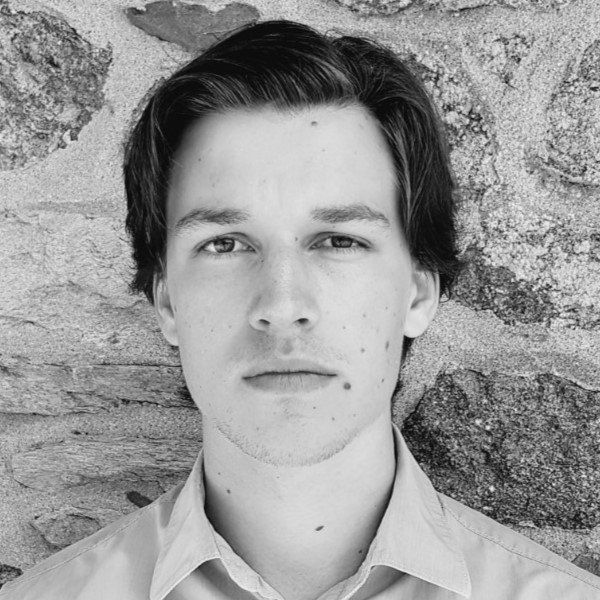
\includegraphics[width=0.5\linewidth]{moi.jpeg} 
            \hspace{0.1\linewidth}
        \end{minipage}%
    \end{center} % End of center environment
}
\makeatother


\newcolumntype{C}[1]{>{\centering\arraybackslash}m{#1}}

\begin{document}


\maketitle

%\section{Domaines de compétence}



%%%%%%%%%%%%%%%%%%%%%%%%%%%%%%%%%%%%%%%%%%%%%%%%%%%%%% DOMAINES DE COMPETENCES %%%%%%%%%%%%%%%%%%%%%%%%%%%%%%%%%%%%%%%%%%%%%%%%%%%%%%%%%%%%%%%%%%%%%%%

\begin{center}
    
\begin{tikzpicture}
        \draw[mainBlue, line width=1pt] (-0.4\linewidth,-2pt) -- (0.4\linewidth,-2pt);
    \end{tikzpicture}
\end{center}

\begin{tabular}{@{\hspace{0.05\textwidth}}m{0.1\textwidth}@{\hspace{0.05\textwidth}}!{\color{secondaryBlue}\vline width 2pt}@{}m{0.7\textwidth}@{}}
    \textcolor{secondaryBlue}{\textbf{Domaines de compétences}} &
    \begin{itemize}[label={}, topsep=0pt, partopsep=0pt, itemsep=0.5pt, parsep=2pt]
        \setlength{\itemsep}{10pt} 

        \item \textcolor{darkGray}{Hardware - Electronique}
        \begin{itemize}[label={\textcolor{gray!100}{\checkmark}}, topsep=0pt, partopsep=0pt, itemsep=0.5pt, parsep=2pt] 
            \item \textcolor{gray!100}{Conception de schémas électriques, routage, simulation }
            \item \textcolor{gray!100}{Filtrage analogique actif et passif, Matlab}
        \end{itemize}

        \item \textcolor{darkGray}{Electronique numérique} 
        \begin{itemize}[label={\textcolor{gray!100}{\checkmark}}, topsep=0pt, partopsep=0pt, itemsep=0.5pt, parsep=2pt] 
            \item \textcolor{gray!100}{Microcontrôleurs : programmation en C et Assembleur sur Keil-uVision }
            \item \textcolor{gray!100}{Logique programmable : technologie FPGA, description VHDL}
            \item \textcolor{gray!100}{Systèmes sur puce : SoC, SoC-FPGA, SoC-IP}
        \end{itemize}

        \item \textcolor{darkGray}{Informatique}
        \begin{itemize}[label={\textcolor{gray!100}{\checkmark}}, topsep=0pt, partopsep=0pt, itemsep=0.5pt, parsep=2pt] 
            \item \textcolor{gray!100}{Programmation bas-niveau : microcontrôleurs, FreeRTOS}
            \item \textcolor{gray!100}{Informatique industrielle : traitement d'image, création d'interfaces graphiques}
            \item \textcolor{gray!100}{Développement jeux-vidéos}
        \end{itemize}

        \item \textcolor{darkGray}{Ingénierie système}
        \begin{itemize}[label={\textcolor{gray!100}{\checkmark}}, topsep=0pt, partopsep=0pt, itemsep=0.5pt, parsep=2pt, after=\vspace*{-\baselineskip}] % reduce spacing & adjust left margin
            \item \textcolor{gray!100}{Rédaction de cahier des charges}
            \item \textcolor{gray!100}{Etudes de faisabilité}
        \end{itemize}
    \end{itemize}
\end{tabular}


%%%%%%%%%%%%%%%%%%%%%%%%%%%%%%%%%%%%%%%%%%%%%%%%%%%%%% LANGAGES OUTILS NORMES %%%%%%%%%%%%%%%%%%%%%%%%%%%%%%%%%%%%%%%%%%%%%%%%%%%%%%%%%%%%%%%%%%%%%%%

\begin{center}
    
\begin{tikzpicture}
        \draw[mainBlue, line width=1pt] (-0.4\linewidth,-2pt) -- (0.4\linewidth,-2pt);
    \end{tikzpicture}
\end{center}


\begin{tabular}{@{\hspace{0.05\textwidth}}m{0.1\textwidth}@{\hspace{0.05\textwidth}}!{\color{secondaryBlue}\vline width 2pt}@{}m{0.7\textwidth}@{}}
    \textcolor{secondaryBlue}{\textbf{Langages\newline Outils\newline Normes}} & 
    \begin{itemize}[label={}, topsep=0pt, partopsep=0pt, itemsep=0.5pt, parsep=2pt] 

        \item \textcolor{darkGray}{Langages}
        \begin{itemize}[label={\textcolor{gray!100}{\checkmark}}, topsep=0pt, partopsep=0pt, itemsep=0.5pt, parsep=2pt] 
            \item \textcolor{gray!100}{C, C++, Python, Java, Assembleur}
        \end{itemize}

        \item \textcolor{darkGray}{Outils}
        \begin{itemize}[label={\textcolor{gray!100}{\checkmark}}, topsep=0pt, partopsep=0pt, itemsep=0.5pt, parsep=2pt]
            \item \textcolor{gray!100}{Collaboratifs : Git, Jira, Confluence, Teams}
            \item \textcolor{gray!100}{IDEs : VSCode, STM32CubeIDE, Eclipse}
            \item \textcolor{gray!100}{Bibliothèques : OpenCV, PyQt5, NumPy, SFML, Matplotlib, RealSense}
            \item \textcolor{gray!100}{Modélisation : OrCAD PSpice, Visio, Blender, draw.io}
        \end{itemize}

        \item \textcolor{darkGray}{Normes}
        \begin{itemize}[label={\textcolor{gray!100}{\checkmark}}, topsep=0pt, partopsep=0pt, itemsep=0.5pt, parsep=2pt, after=\vspace*{-\baselineskip}] 
            \item \textcolor{gray!100}{ISO7816 (smart-cards), ISO12233 (traitement d'image)}
        \end{itemize}
    \end{itemize}
\end{tabular}


%%%%%%%%%%%%%%%%%%%%%%%%%%%%%%%%%%%%%%%%%%%%%%%%%%%%%% SECTEURS D'ACTIVITES %%%%%%%%%%%%%%%%%%%%%%%%%%%%%%%%%%%%%%%%%%%%%%%%%%%%%%%%%%%%%%%%%%%%%%%

\begin{center}
    
\begin{tikzpicture}
        \draw[mainBlue, line width=1pt] (-0.4\linewidth,-2pt) -- (0.4\linewidth,-2pt);
    \end{tikzpicture}
\end{center}


\begin{tabular}{@{\hspace{0.05\textwidth}}m{0.1\textwidth}@{\hspace{0.05\textwidth}}!{\color{secondaryBlue}\vline width 2pt}@{}C{0.7\textwidth}@{}}
    \textcolor{secondaryBlue}{\textbf{Secteurs d'activités}} & 
    \begin{itemize}[label={}, topsep=0pt, partopsep=0pt, itemsep=0.5pt, parsep=2pt, after=\vspace*{-\baselineskip}]
        \item \textcolor{gray!100}{Systèmes d'identification et de sécurité}
        \item \textcolor{gray!100}{Systèmes d'acquisition automatisés}
        \item \textcolor{gray!100}{Smart-Cards}
    \end{itemize}
\end{tabular}


%%%%%%%%%%%%%%%%%%%%%%%%%%%%%%%%%%%%%%%%%%%%%%%%%%%%%% FORMATION %%%%%%%%%%%%%%%%%%%%%%%%%%%%%%%%%%%%%%%%%%%%%%%%%%%%%%%%%%%%%%%%%%%%%%%

\begin{center}
    
\begin{tikzpicture}
        \draw[mainBlue, line width=1pt] (-0.4\linewidth,-2pt) -- (0.4\linewidth,-2pt);
    \end{tikzpicture}
\end{center}


\begin{tabular}{@{\hspace{0.05\textwidth}} m{0.1\textwidth} @ {\hspace{0.05\textwidth}} ! {\color{secondaryBlue}\vline width 2pt \hspace{0.04\textwidth}} @ {}m{0.4\textwidth} @{\hspace{0.15\textwidth}} m{0.5\linewidth}@{}}
    \textcolor{secondaryBlue}{\textbf{Formation}} & 
    \textcolor{darkGray}{Ingénieur électronicien ENSEA}
    \begin{itemize}[label={\textcolor{gray!100}{\checkmark}}, topsep=0pt, partopsep=0pt, itemsep=0.5pt, parsep=2pt, after=\vspace*{-\baselineskip}]
        \item \textcolor{gray!100}{Année d'obtention du diplôme : 2023} 
        \item \textcolor{gray!100}{Spécialités : microélectronique et numérique} 
    \end{itemize} &
    
\includegraphics[width=0.1\linewidth]{ensea.jpg}
\end{tabular}


%%%%%%%%%%%%%%%%%%%%%%%%%%%%%%%%%%%%%%%%%%%%%%%%%%%%%% LANGUES %%%%%%%%%%%%%%%%%%%%%%%%%%%%%%%%%%%%%%%%%%%%%%%%%%%%%%%%%%%%%%%%%%%%%%%

\begin{center}
    
\begin{tikzpicture}
        \draw[mainBlue, line width=1pt] (-0.4\linewidth,-2pt) -- (0.4\linewidth,-2pt);
    \end{tikzpicture}
\end{center}

\begin{tabular}{@{\hspace{0.05\textwidth}}m{0.1\textwidth}@{\hspace{0.05\textwidth}}!{\color{secondaryBlue}\vline width 2pt}@{}C{0.7\textwidth}@{}}
    \textcolor{secondaryBlue}{\textbf{Langues}} & 
    \begin{itemize}[label={}, topsep=0pt, partopsep=0pt, itemsep=0.5pt, parsep=2pt, after=\vspace*{-\baselineskip}]
        \item \textcolor{gray!100}{Anglais : bilingue (915/990 à l'examen TOEIC)}
        \item \textcolor{gray!100}{Français : langue maternelle}
    \end{itemize}
\end{tabular}

%%%%%%%%%%%%%%%%%%%%%%%%%%%%%%%%%%%%%%%%%%%%%%%%%%%%%%%%%%%%%% EXPERIENCE IDEMIA %%%%%%%%%%%%%%%%%%%%%%%%%%%%%%%%%%%%%%%%%%%%%%%%%%%%%%%%%%%%%%%%%%%%%%%%%
\newpage
\fancypagestyle{pro_experience_idemia}
{
    \fancyhf{} 
    \fancyhead[L] % Left header
    {
        \vspace*{10pt} % Adjust vertical space as needed
        \textcolor{darkGray}{Dossier de compétences } 
    } 
    \fancyhead[C] % Central header
    {
        \vspace*{10pt} % Adjust vertical space as needed
        \textcolor{darkGray}{\textbf{Expériences professionnelles}}
    } 
    \fancyhead[R]
    {
        \vspace*{10pt} % Adjust vertical space as needed
        \begin{minipage}[b]{2cm}
            \raisebox{-1.25\height}{
\includegraphics[width=2cm]{logo_idemia.jpg}}
        \end{minipage}
        \hspace{25pt}
        \begin{minipage}[b]{2cm}
            \raisebox{-1\height}{
\includegraphics[width=0.75cm]{ensea.jpg}}
        \end{minipage}
    } 
    \fancyfoot[C]{\thepage\ / \pageref{LastPage}} % Center footer with page number / total number of pages
    \renewcommand{\headrulewidth}{2pt} % Header rule width
    \renewcommand{\headrule}{\color{mainBlue}\hrule width\headwidth height\headrulewidth \vskip-\headrulewidth} % Redefine color of header rule
}
\thispagestyle{pro_experience_idemia}


\vspace*{0cm} % Vertical space from the top of the page

\vfill % Stretchable vertical space to center vertically the whole page

\begin{center}
    \textcolor{secondaryBlue}{\textbf{Projet ALIX}}
\end{center}


\begin{tabular}
    {
        @{}m{0.1\textwidth}
        @{\hspace{0.001\textwidth}}!{\color{secondaryBlue}\vline width 2pt}
        @{}m{0.5\textwidth}
        @{\hspace{0.025\textwidth}}!{\color{secondaryBlue}\vline width 2pt}
        @{}m{0.3\textwidth}
    }
    \textcolor{secondaryBlue}{\textbf{Description}}           
    &
    \begin{itemize}[label={}, topsep=8pt, partopsep=0pt, itemsep=0.5pt, parsep=2pt, after=\vspace*{-\baselineskip}]
        \setlength{\itemsep}{10pt} 
        \item \textcolor{darkGray}{Informations projet}
        \begin{itemize}[label={\textcolor{gray!100}{\checkmark}}, topsep=8pt, partopsep=0pt, itemsep=0.5pt, parsep=2pt] 
            \item \textcolor{gray!100}{ALIX : Augmented Luggage Identity eXperience}
            \item \textcolor{gray!100}{Partenariat Air France}
            \item \textcolor{gray!100}{Système multi-caméras avec éclairage LED synchronisé}
            \item \textcolor{gray!100}{Aide à retrouver les bagages perdus sans étiquette}
            \begin{itemize}
                [label={\textcolor{gray!100}{$\triangleright$}}, topsep=0pt, partopsep=0pt, itemsep=0.5pt, parsep=2pt] 
                \item \textcolor{gray!100}{Acquisition du bagage en temps réel}
                \item \textcolor{gray!100}{Envoi des images dans la base de données}
                \item \textcolor{gray!100}{Appairage dans le backend grâce à l'I.A}
            \end{itemize}
        \end{itemize}
    \end{itemize}
    &
    \begin{itemize}[label={}, topsep=8pt, partopsep=0pt, itemsep=0.5pt, parsep=2pt, after=\vspace*{-\baselineskip}]
        \setlength{\itemsep}{10pt} 
        \item \textcolor{darkGray}{Ma contribution}
        \begin{itemize}[label={\textcolor{gray!100}{\checkmark}}, topsep=8pt, partopsep=0pt, itemsep=0.5pt, parsep=2pt] 
            \item \textcolor{gray!100}{Rôle : ingénieur apprenti}
            \item \textcolor{gray!100}{Pilote industriel : Jan. 2021 à Jan. 2022 (2 ans)}
            \item \textcolor{gray!100}{Industrialisation : Jan. 2022 à Juil. 2023 (7 mois)}
            \item \textcolor{gray!100}{Système d'acquisition}
            \item \textcolor{gray!100}{Banc industriel de calibration des caméras}
            %\item[\textcolor{white}{\checkmark}] \textcolor{gray!100}{} % ghost item
        \end{itemize}
    \end{itemize}
\end{tabular}

\begin{center}
    
\begin{tikzpicture}
        \draw[mainBlue, line width=1pt] (-0.45\linewidth,-2pt) -- (0.45\linewidth,-2pt);
    \end{tikzpicture}
\end{center}

%%%%%%%%%%%%%%%%%%%%%%%%%%%%%% HARDWARE - ELECTRONIQUE
\begin{tabular}
    {
        @{}m{0.1\textwidth}
        @{\hspace{0.001\textwidth}}!{\color{secondaryBlue}\vline width 2pt}
        @{}m{0.5\textwidth}
        @{\hspace{0.025\textwidth}}!{\color{secondaryBlue}\vline width 2pt}
        @{}m{0.3\textwidth}
    }
    \textcolor{secondaryBlue}{\textbf{Hardware Electronique}}           
    &
    \begin{itemize}[label={}, topsep=8pt, partopsep=0pt, itemsep=0.5pt, parsep=2pt, after=\vspace*{-\baselineskip}]
        \setlength{\itemsep}{10pt} 
        \item \textcolor{darkGray}{Tâches}
        \begin{itemize}[label={\textcolor{gray!100}{$\checkmark$}}, topsep=8pt, partopsep=0pt, itemsep=0.5pt, parsep=2pt] 
            \item \textcolor{gray!100}{Mise en place de la solution d'éclairage}
            \begin{itemize}[label={\textcolor{gray!100}{$\triangleright$}}, topsep=0pt, partopsep=0pt, itemsep=0.5pt, parsep=2pt] 
                \item \textcolor{gray!100}{Recherche de matériel existant}
                \item \textcolor{gray!100}{Validation par mesure de la puissance lumineuse}
                \item \textcolor{gray!100}{Validation par mesure de la fréquence des flashs}
                \item \textcolor{gray!100}{Analyse du mode de fonctionnement sécuritaire}
                \item \textcolor{gray!100}{Adaptation d'un driver d'éclairage IDEMIA existant}
                \item \textcolor{gray!100}{Déploiement du firmware sur les drivers}
            \end{itemize}
            \item \textcolor{gray!100}{Création des schémas de connexion des signaux du système}
            \item \textcolor{gray!100}{Estimation précise des besoins énergétiques}
            
        \end{itemize}
    \end{itemize}
    &
    \begin{itemize}[label={}, topsep=8pt, partopsep=0pt, itemsep=0.5pt, parsep=2pt, after=\vspace*{-\baselineskip}]
        \setlength{\itemsep}{10pt} 
        \item \textcolor{darkGray}{Outils}
        \begin{itemize}[label={\textcolor{gray!100}{\checkmark}}, topsep=8pt, partopsep=0pt, itemsep=0.5pt, parsep=2pt] 
            \item \textcolor{gray!100}{LTSpice}
            \item \textcolor{gray!100}{Oscilloscopes (Lecroy)}
            \item \textcolor{gray!100}{Luxmètre}
            \item \textcolor{gray!100}{Logiciel de visualisation de PCB}
            \item \textcolor{gray!100}{GBF, alimentations électriques}
            \item \textcolor{gray!100}{Logiciel de dessin Visio}
            \item \textcolor{gray!100}{STM32CubeProgrammer}
            \item[\textcolor{white}{\checkmark}] \textcolor{gray!100}{} % ghost item
            \item[\textcolor{white}{\checkmark}] \textcolor{gray!100}{} % ghost item
        \end{itemize}
    \end{itemize}
\end{tabular}

\begin{center}
    
\begin{tikzpicture}
        \draw[mainBlue, line width=1pt] (-0.45\linewidth,-2pt) -- (0.45\linewidth,-2pt);
    \end{tikzpicture}
\end{center}

%%%%%%%%%%%%%%%%%%%%%%%%%%%%%%%%% INFORMATIQUE

\begin{tabular}
    {
        @{}m{0.1\textwidth}
        @{\hspace{0.001\textwidth}}!{\color{secondaryBlue}\vline width 2pt} % not a column
        @{}m{0.5\textwidth}
        @{\hspace{0.025\textwidth}}!{\color{secondaryBlue}\vline width 2pt} % not a column
        @{{\hspace{0.001\textwidth}}}m{0.3\textwidth}
    }
    \textcolor{secondaryBlue}
    {
        \textbf{Informatique}
    }           
    &
    \begin{itemize}
        [label={}, topsep=8pt, partopsep=0pt, itemsep=0.5pt, parsep=2pt,after=\vspace*{-\baselineskip}]
        \setlength{\itemsep}{10pt} 

        \item \textcolor{darkGray}{Tâches} 
        \begin{itemize}
        [label={\textcolor{gray!100}{\checkmark}}, topsep=8pt, partopsep=0pt, itemsep=0.5pt, parsep=2pt] 
            \item \textcolor{gray!100}{Recherche et test du capteur détecteur de bagages}
            \item \textcolor{gray!100}{Modélisation 3D du système d'acquisition}
            \begin{itemize}
                [label={\textcolor{gray!100}{$\triangleright$}}, topsep=0pt, partopsep=0pt, itemsep=0.5pt, parsep=2pt]
                \item \textcolor{gray!100}{Simulation des champs vision caméras}
                \item \textcolor{gray!100}{Réduction de la longueur du système}
                \item \textcolor{gray!100}{Réduction des reflets sur l'image}
            \end{itemize}
            \item \textcolor{gray!100}{Conversion de code Python vers C++}
            \item \textcolor{gray!100}{Traitement d'image : optimisation du SNR des caméras}
            \item \textcolor{gray!100}{Réalisation d'un banc industriel de calibration des caméras}
            \begin{itemize}
            [label={\textcolor{gray!100}{$\triangleright$}}, topsep=0pt, partopsep=0pt, itemsep=0.5pt, parsep=2pt]   
                \item \textcolor{gray!100}{Intégration d'algorithmes de mesure de netteté (MTF) }
                \item \textcolor{gray!100}{Intégration de l'algorithme de balance des blancs}
                \item \textcolor{gray!100}{Développement de la détection automatique des mires}
                \item \textcolor{gray!100}{Création des requètes HTTP associées}
            \end{itemize}
        \end{itemize}
    \end{itemize}
    &
    \begin{itemize}[label={}, topsep=8pt, partopsep=0pt, itemsep=0.5pt, parsep=2pt,after=\vspace*{-\baselineskip}]
        \setlength{\itemsep}{10pt} 
        \item \textcolor{darkGray}{Environnement, normes et outils} 
        \begin{itemize}
        [label={\textcolor{gray!100}{\checkmark}}, topsep=8pt, partopsep=0pt, itemsep=0.5pt, parsep=2pt] 
            \item \textcolor{gray!100}{ARM / Linux Debian}
            \item \textcolor{gray!100}{Blender}
            \item \textcolor{gray!100}{Norme ISO 12233}
            \item \textcolor{gray!100}{OpenCV pour C++}
            \item \textcolor{gray!100}{VSCode, SSH, SVN, CMake}
            \item \textcolor{gray!100}{Compilation croisée (schroot)}
            \item \textcolor{gray!100}{ArUco}
            \item \textcolor{gray!100}{cpp-httplib} 
            \item[\textcolor{white}{\checkmark}] \textcolor{gray!100}{} % ghost item
            \item[\textcolor{white}{\checkmark}] \textcolor{gray!100}{} % ghost item
            \item[\textcolor{white}{\checkmark}] \textcolor{gray!100}{} % ghost item
            \item[\textcolor{white}{\checkmark}] \textcolor{gray!100}{} % ghost item
        \end{itemize}
    \end{itemize}
\end{tabular}

\begin{center}
    
\begin{tikzpicture}
        \draw[mainBlue, line width=1pt] (-0.45\linewidth,-2pt) -- (0.45\linewidth,-2pt);
    \end{tikzpicture}
\end{center}

%%%%%%%%%%%%%%%%%%%%%%%%%%%%%%%% GESTION DE PROJET %%%%%%%%%%%%%%%%%

\begin{tabular}
    {
        @{}m{0.1\textwidth}
        @{\hspace{0.001\textwidth}}!{\color{secondaryBlue}\vline width 2pt} % not a column
        @{}m{0.5\textwidth}
        @{\hspace{0.025\textwidth}}!{\color{secondaryBlue}\vline width 2pt} % not a column
        @{{\hspace{0.001\textwidth}}}m{0.3\textwidth}
    }
    \textcolor{secondaryBlue}
    {
        \textbf{Projet}
    } 

    &
    \begin{itemize}
        [label={}, topsep=8pt, partopsep=0pt, itemsep=0.5pt, parsep=2pt,after=\vspace*{-\baselineskip}]
        \setlength{\itemsep}{10pt}
        \item \textcolor{darkGray}{Tâches}
        \begin{itemize}
        [label={\textcolor{gray!100}{\checkmark}}, topsep=8pt, partopsep=0pt, itemsep=0.5pt, parsep=2pt, after=\vspace*{-\baselineskip}] 
            \item \textcolor{gray!100}{Modification du cahier des charges pour le pilote industriel}
            \item \textcolor{gray!100}{Conception du banc industriel de calibration caméra}
            \begin{itemize}
                [label={\textcolor{gray!100}{$\triangleright$}}, topsep=0pt, partopsep=0pt, itemsep=0.5pt, parsep=2pt]
                \item \textcolor{gray!100}{Rédaction du cahier des charges}
                \item \textcolor{gray!100}{Planification des tâches}
                \item \textcolor{gray!100}{Diagramme d'interfaces systèmes IDEMIA et client}
                \item \textcolor{gray!100}{Rédaction du manuel d'utilisation client}  
                \item \textcolor{gray!100}{Soutenance du projet devant IDEMIA et mon école}
            \end{itemize}
        \end{itemize}
    \end{itemize}
    &
    \begin{itemize}
        [label={}, topsep=8pt, partopsep=0pt, itemsep=0.5pt, parsep=2pt,after=\vspace*{-\baselineskip}]
        \setlength{\itemsep}{10pt}
        \item \textcolor{darkGray}{Outils}
        \begin{itemize}
        [label={\textcolor{gray!100}{\checkmark}}, topsep=8pt, partopsep=0pt, itemsep=0.5pt, parsep=2pt,after=\vspace*{-\baselineskip}] 
            \item \textcolor{gray!100}{Word, Excel}
            \item \textcolor{gray!100}{Diagramme de Gantt}
            \item \textcolor{gray!100}{Logiciel de schématique draw.io}
            \item[\textcolor{white}{\checkmark}] \textcolor{gray!100}{} % ghost item
            \item[\textcolor{white}{\checkmark}] \textcolor{gray!100}{} % ghost item
            \item[\textcolor{white}{\checkmark}] \textcolor{gray!100}{} % ghost item
            \item[\textcolor{white}{\checkmark}] \textcolor{gray!100}{} % ghost item
        \end{itemize}
    \end{itemize}
\end{tabular}

\vfill % Stretchable vertical space

%%%%%%%%%%%%%%%%%%%%%%%%%%%%%%%%%%%%%%%%%%%%%% EXPERIENCE ICE-TECH / LINXENS  %%%%%%%%%%%%%%%%%%%%%%%%%%%%%%%%%%%%%%%%%%%%%%%%%%%%%%%%%%%%%%%%%%%%%%%%%

\newpage

\fancypagestyle{pro_experience_linxens}
{
    \fancyhf{} 
    \fancyhead[L] % Left header
    {
        \vspace*{10pt} % Adjust vertical space as needed
        \textcolor{darkGray}{Dossier de compétences } 
    } 
    \fancyhead[C] % Central header 
    {
        \vspace*{10pt} % Adjust vertical space as needed
        \textcolor{darkGray}{\textbf{Expériences professionnelles}}
    } 

    \fancyhead[R]
    {
        \vspace*{10pt} % Adjust vertical space as needed
        \begin{minipage}[b]{2cm}
            \raisebox{-1.15\height}{
\includegraphics[width=3cm]{logo_linxens.jpg}}
        \end{minipage}
        \hspace{50pt}
        \begin{minipage}[b]{2cm}
            \raisebox{-1\height}{
\includegraphics[width=2cm]{logo_ice-tech.png}}
        \end{minipage}
    } 
    \fancyfoot[C]{\thepage\ / \pageref{LastPage}} % Center footer with page number / total number of pages
    \renewcommand{\headrulewidth}{2pt} % Header rule width
    \renewcommand{\headrule}{\color{mainBlue}\hrule width\headwidth height\headrulewidth \vskip-\headrulewidth} % Redefine color of header rule
}

\thispagestyle{pro_experience_linxens}

\vspace*{0cm}

\vfill % Stretchable vertical space to center vertically the whole page

\begin{center}
    \textcolor{secondaryBlue}{\textbf{Ingénieur responsable du test électrique des produits biométriques}}
\end{center}

\vspace*{1cm}

\begin{tabular}
    {
        @{}m{0.1\textwidth}
        @{\hspace{0.001\textwidth}}!{\color{secondaryBlue}\vline width 2pt}
        @{}m{0.5\textwidth}
        @{\hspace{0.025\textwidth}}!{\color{secondaryBlue}\vline width 2pt}
        @{}m{0.3\textwidth}
    }
    \textcolor{secondaryBlue}{\textbf{Description}}           
    &
    \begin{itemize}[label={}, topsep=8pt, partopsep=0pt, itemsep=0.5pt, parsep=2pt, after=\vspace*{-\baselineskip}]
        \setlength{\itemsep}{10pt} 
        \item \textcolor{darkGray}{Informations}
        \begin{itemize}[label={\textcolor{gray!100}{\checkmark}}, topsep=8pt, partopsep=0pt, itemsep=0.5pt, parsep=2pt] 
            \item \textcolor{gray!100}{Site de Buchelay (78)}
            \item \textcolor{gray!100}{Secteur des cartes à puces}
            \item \textcolor{gray!100}{Environnement salle blanche}
            \item \textcolor{gray!100}{Test électrique}
            \begin{itemize}
                [label={\textcolor{gray!100}{$\triangleright$}}, topsep=0pt, partopsep=0pt, itemsep=0.5pt, parsep=2pt] 
                \item \textcolor{gray!100}{Vérification finale de conformité avant envoi au client}
                \item \textcolor{gray!100}{Système industriel à grande capacité de production}
            \end{itemize}
            %\item[\textcolor{white}{}] {} % ghost item
        \end{itemize}
    \end{itemize}
    &
    \begin{itemize}[label={}, topsep=8pt, partopsep=0pt, itemsep=0.5pt, parsep=2pt, after=\vspace*{-\baselineskip}]
        \setlength{\itemsep}{10pt} 
        \item \textcolor{darkGray}{Ma contribution}
        \begin{itemize}[label={\textcolor{gray!100}{\checkmark}}, topsep=8pt, partopsep=0pt, itemsep=0.5pt, parsep=2pt] 
            \item \textcolor{gray!100}{Jan. 2024 à aujourd'hui (5 mois)}
            \item \textcolor{gray!100}{Automatisation de l'analyse de la qualité}
            \item \textcolor{gray!100}{Documentation}
            \item \textcolor{gray!100}{Amélioration du positionnement}
            \item \textcolor{gray!100}{Support en production}
        \end{itemize}
    \end{itemize}
\end{tabular}

\begin{center}
    
\begin{tikzpicture}
        \draw[mainBlue, line width=1pt] (-0.45\linewidth,-2pt) -- (0.45\linewidth,-2pt);
    \end{tikzpicture}
\end{center}


%%%%%%%%%%%%%%%%%%%%%%%%%%%%%%%%% INFORMATIQUE

\begin{tabular}
    {
        @{}m{0.1\textwidth}
        @{\hspace{0.001\textwidth}}!{\color{secondaryBlue}\vline width 2pt} % not a column
        @{}m{0.5\textwidth}
        @{\hspace{0.025\textwidth}}!{\color{secondaryBlue}\vline width 2pt} % not a column
        @{{\hspace{0.001\textwidth}}}m{0.3\textwidth} 
    }
    \textcolor{secondaryBlue}
    {
        \textbf{Informatique}
    }           
    &
    \begin{itemize}
        [label={}, topsep=8pt, partopsep=0pt, itemsep=0.5pt, parsep=2pt,after=\vspace*{-\baselineskip}]
        \setlength{\itemsep}{10pt} 

        \item \textcolor{darkGray}{Tâches} 
        \begin{itemize}
        [label={\textcolor{gray!100}{\checkmark}}, topsep=8pt, partopsep=0pt, itemsep=0.5pt, parsep=2pt] 
            \item \textcolor{gray!100}{Développement intégral d'un logiciel d'analyse de la qualité}
            \begin{itemize}
                [label={\textcolor{gray!100}{$\triangleright$}}, topsep=0pt, partopsep=0pt, itemsep=0.5pt, parsep=2pt]
                \item \textcolor{gray!100}{Analyse des informations contenues dans les logfiles de la machine de test électrique}
                \item \textcolor{gray!100}{Algorithmes de parsing pour différents formats}
                \item \textcolor{gray!100}{Algorithmes de visualisation des données}
                \item \textcolor{gray!100}{Refactorisation en bibliothèque orientée objet (OOP)}
                \item \textcolor{gray!100}{Interface utilisateur graphique et ergonomique}
                \item \textcolor{gray!100}{Documentations utilisateur et développeur}
            \end{itemize}
            \item \textcolor{gray!100}{Amélioration de programmes de reconnaissance visuelle}
        \end{itemize}
        \item \textcolor{darkGray}{Formations} 
        \begin{itemize}
            [label={\textcolor{gray!100}{\checkmark}}, topsep=8pt, partopsep=0pt, itemsep=0.5pt, parsep=2pt] 
                \item \textcolor{gray!100}{Logiciel de reconnaissance visuelle des smart-cards}
                \item \textcolor{gray!100}{Bases de la cybersecurité des smart-cards}
        \end{itemize}
    \end{itemize}
    &
    \begin{itemize}[label={}, topsep=8pt, partopsep=0pt, itemsep=0.5pt, parsep=2pt,after=\vspace*{-\baselineskip}]
        \setlength{\itemsep}{10pt} 
        \item \textcolor{darkGray}{Environnement, normes et outils} 
        \begin{itemize}
        [label={\textcolor{gray!100}{\checkmark}}, topsep=8pt, partopsep=0pt, itemsep=0.5pt, parsep=2pt] 
            \item \textcolor{gray!100}{Norme ISO 7816}
            \item \textcolor{gray!100}{Python 3.12}
            \item \textcolor{gray!100}{NumPy}
            \item \textcolor{gray!100}{Matplotlib}
            \item \textcolor{gray!100}{PyQt5}
            \item[\textcolor{white}{\checkmark}] \textcolor{gray!100}{} % ghost item
            \item[\textcolor{white}{\checkmark}] \textcolor{gray!100}{} % ghost item
            \item[\textcolor{white}{\checkmark}] \textcolor{gray!100}{} % ghost item
            \item[\textcolor{white}{\checkmark}] \textcolor{gray!100}{} % ghost item
            \item[\textcolor{white}{\checkmark}] \textcolor{gray!100}{} % ghost item
            \item[\textcolor{white}{\checkmark}] \textcolor{gray!100}{} % ghost item
            \item[\textcolor{white}{\checkmark}] \textcolor{gray!100}{} % ghost item
            \item[\textcolor{white}{\checkmark}] \textcolor{gray!100}{} % ghost item
        \end{itemize}
    \end{itemize}
\end{tabular}

\begin{center}
    
\begin{tikzpicture}
        \draw[mainBlue, line width=1pt] (-0.45\linewidth,-2pt) -- (0.45\linewidth,-2pt);
    \end{tikzpicture}
\end{center}

%%%%%%%%%%%%%%%%%%%%%%%%%%%%%%%% GESTION DE PROJET %%%%%%%%%%%%%%%%%

\begin{tabular}
    {
        @{}m{0.1\textwidth}
        @{\hspace{0.001\textwidth}}!{\color{secondaryBlue}\vline width 2pt} % not a column
        @{}m{0.5\textwidth}
        @{\hspace{0.025\textwidth}}!{\color{secondaryBlue}\vline width 2pt} % not a column
        @{{\hspace{0.001\textwidth}}}m{0.3\textwidth}
    }
    \textcolor{secondaryBlue}
    {
        \textbf{Support}
    } 

    &
    \begin{itemize}
        [label={}, topsep=8pt, partopsep=0pt, itemsep=0.5pt, parsep=2pt,after=\vspace*{-\baselineskip}]
        \setlength{\itemsep}{10pt}
        \item \textcolor{darkGray}{Tâches}
        \begin{itemize}
        [label={\textcolor{gray!100}{\checkmark}}, topsep=8pt, partopsep=0pt, itemsep=0.5pt, parsep=2pt, after=\vspace*{-\baselineskip}] 

            \item \textcolor{gray!100}{Résolution de panne complexe empêchant la production}
            \begin{itemize}
                [label={\textcolor{gray!100}{$\triangleright$}}, topsep=0pt, partopsep=0pt, itemsep=0.5pt, parsep=2pt]
                \item \textcolor{gray!100}{Rédaction d'un plan d'action pour la résolution}
                \item \textcolor{gray!100}{Mise en oeuvre de mesures préventives}
                \item \textcolor{gray!100}{Documentation du procédé établi}
            \end{itemize}
            \item \textcolor{gray!100}{Apprentissage du fonctionnement de la machine}
            \item \textcolor{gray!100}{Supervision lors du lancement d'un nouveau produit}
            \item \textcolor{gray!100}{Fiabilisation du procédé de positionnement}
            \begin{itemize}
                [label={\textcolor{gray!100}{$\triangleright$}}, topsep=0pt, partopsep=0pt, itemsep=0.5pt, parsep=2pt]
                \item \textcolor{gray!100}{Documentation du fonctionnement du positionnement}
                \item \textcolor{gray!100}{Réunions de travail avec différents départements}
            \end{itemize}
            \item \textcolor{gray!100}{Documentation à destination des opérateurs}
            \begin{itemize}
            [label={\textcolor{gray!100}{$\triangleright$}}, topsep=0pt, partopsep=0pt, itemsep=0.5pt, parsep=2pt]
                \item \textcolor{gray!100}{Guides de dépannage}
                \item \textcolor{gray!100}{Fiches d'instructions produit}
            \end{itemize}
        \end{itemize}
    \end{itemize}
    &
    \begin{itemize}
        [label={}, topsep=8pt, partopsep=0pt, itemsep=0.5pt, parsep=2pt,after=\vspace*{-\baselineskip}]
        \setlength{\itemsep}{10pt}
        \item \textcolor{darkGray}{Outils}
        \begin{itemize}
        [label={\textcolor{gray!100}{\checkmark}}, topsep=8pt, partopsep=0pt, itemsep=0.5pt, parsep=2pt,after=\vspace*{-\baselineskip}] 
            \item \textcolor{gray!100}{Word, Excel}
            \item \textcolor{gray!100}{Logiciel de reconnaissance visuelle des produits}
            \item \textcolor{gray!100}{Logiciel de test électrique}
            \item \textcolor{gray!100}{Logiciel de dessin draw.io}
            \item \textcolor{gray!100}{Caméra à vision microscopique}
            \item[\textcolor{white}{\checkmark}] \textcolor{gray!100}{} % ghost item
            \item[\textcolor{white}{\checkmark}] \textcolor{gray!100}{} % ghost item
            \item[\textcolor{white}{\checkmark}] \textcolor{gray!100}{} % ghost item
            \item[\textcolor{white}{\checkmark}] \textcolor{gray!100}{} % ghost item
            \item[\textcolor{white}{\checkmark}] \textcolor{gray!100}{} % ghost item
            \item[\textcolor{white}{\checkmark}] \textcolor{gray!100}{} % ghost item



        \end{itemize}
    \end{itemize}
\end{tabular}

\vfill % Stretchable vertical space


%%%%%%%%%%%%%%%%%%%%%%%%%%%%%%%%%%%%%%% STUDENT LAB WORK %%%%%%%%%%%%%%%%%%%%%%%%%%%%%%%%%%%%%%%


\newpage

\fancypagestyle{student_lab_work_ENSEA}
{
    \fancyhf{} 
    \fancyhead[L] % Left header
    {
        \vspace*{10pt} % Adjust vertical space as needed
        \textcolor{darkGray}{Dossier de compétences} 
    } 
    \fancyhead[C] % Central header 
    {
        \vspace*{10pt} % Adjust vertical space as needed
        \textcolor{darkGray}{\textbf{Travaux Pratiques ENSEA}}
    } 
    \fancyhead[R]
    {
        \vspace*{10pt} % Adjust vertical space as needed
        \raisebox{-1\height}{
\includegraphics[width=0.8cm]{ensea.jpg}}
    } 
    \fancyfoot[C]{\thepage\ / \pageref{LastPage}} % Center footer with page number / total number of pages
    \renewcommand{\headrulewidth}{2pt} % Header rule width
    \renewcommand{\headrule}{\color{mainBlue}\hrule width\headwidth height\headrulewidth \vskip-\headrulewidth} % Redefine color of header rule
}

\thispagestyle{student_lab_work_ENSEA}

\vspace*{0cm}

\vfill % Stretchable vertical space to center vertically the whole page


%%%%%%%%%%%%%%%%%%%%%%%%%%%%%%%%%%%%%% TP SOC FPGA %%%%%%%%%%%%

\begin{tabular}
{
    @{}m{0.1\textwidth}
    @{\hspace{0.001\textwidth}}!{\color{secondaryBlue}\vline width 2pt} % not a column
    @{}m{0.5\textwidth}
    @{\hspace{0.025\textwidth}}!{\color{secondaryBlue}\vline width 2pt} % not a column
    @{{\hspace{0.001\textwidth}}}m{0.3\textwidth}
}
\textcolor{secondaryBlue}
{
    \textbf{SoC FPGA}
} 
&
\begin{itemize}[label={}, topsep=8pt,partopsep=0pt, itemsep=0.5pt,parsep=2pt,after=\vspace*{-\baselineskip}] 
    \setlength{\itemsep}{1pt}
    \item \textcolor{darkGray}{Création d'une IP softcore pour contrôler un afficheur 7 segments}
    \begin{itemize}
    [label={\textcolor{gray!100}{\checkmark}},topsep=8pt,partopsep=0pt,itemsep=0.5pt,parsep=2pt,
     after=\vspace*{-\baselineskip}] 
        \item \textcolor{gray!100}{Polling}
        \item \textcolor{gray!100}{Interruptions}
        \item \textcolor{gray!100}{Création d'une IP hardware dédiée}
    \end{itemize}
\end{itemize}
&
\begin{itemize}
    [label={}, topsep=8pt, partopsep=0pt, itemsep=0.5pt, parsep=2pt,after=\vspace*{-\baselineskip}]
    \setlength{\itemsep}{10pt}
    \item \textcolor{darkGray}{Outils}
    \begin{itemize}[label={\textcolor{gray!100}{\checkmark}}, topsep=8pt, 
        partopsep=0pt, itemsep=0.5pt, parsep=2pt, after=\vspace*{-\baselineskip}] 
        
        \item \textcolor{gray!100}{Vivado}
        \item \textcolor{gray!100}{Vivado SDK}
        \item \textcolor{gray!100}{ModelSim}
        \item \textcolor{gray!100}{Langage C}
        \item \textcolor{gray!100}{Langage VHDL}
        \item \textcolor{gray!100}{Processeur MicroBlaze}
        \item[\textcolor{white}{\checkmark}] \textcolor{gray!100}{} % ghost item

    \end{itemize}
\end{itemize}
\end{tabular}

%%%%%%%%%%%%%%%%%%%%%%%%%%%%%%%%%%%%% TP JAVA %%%%%%%%%%%%%%%%%%%%%

\begin{center}
    
\begin{tikzpicture}
        \draw[mainBlue, line width=1pt] (-0.45\linewidth,-2pt) -- (0.45\linewidth,-2pt);
    \end{tikzpicture}
\end{center}

\begin{tabular}
    {
        @{}m{0.1\textwidth}
        @{\hspace{0.001\textwidth}}!{\color{secondaryBlue}\vline width 2pt} % not a column
        @{}m{0.5\textwidth}
        @{\hspace{0.025\textwidth}}!{\color{secondaryBlue}\vline width 2pt} % not a column
        @{{\hspace{0.001\textwidth}}}m{0.3\textwidth}
    }
    \textcolor{secondaryBlue}
    {
        \textbf{Java}
    } 

    &
    \begin{itemize}
        [label={}, topsep=8pt, partopsep=0pt, itemsep=0.5pt, parsep=2pt,after=\vspace*{-\baselineskip}]
        \setlength{\itemsep}{10pt}
        \item \textcolor{darkGray}{Réalisations}
        \begin{itemize}
        [label={\textcolor{gray!100}{\checkmark}}, topsep=8pt, partopsep=0pt, itemsep=0.5pt, parsep=2pt, after=\vspace*{-\baselineskip}] 

            \item \textcolor{gray!100}{Utilitaire permettant d'indiquer l'aéroport le plus proche du lieu cliqué sur une représentation du globe terrestre}
            \begin{itemize}
                [label={\textcolor{gray!100}{$\triangleright$}}, topsep=0pt, partopsep=0pt, itemsep=0.5pt, parsep=2pt]
                \item \textcolor{gray!100}{Extraction de données à partir d'un fichier CSV}
                \item \textcolor{gray!100}{Représentation du globe terrestre en 3D en rotation sur lui-même}
                \item \textcolor{gray!100}{Algorithme de calcul de distance entre deux points de la surface terrestre}

            \end{itemize}
        \end{itemize}
    \end{itemize}
    &
    \begin{itemize}
        [label={}, topsep=8pt, partopsep=0pt, itemsep=0.5pt, parsep=2pt,after=\vspace*{-\baselineskip}]
        \setlength{\itemsep}{10pt}
        \item \textcolor{darkGray}{Outils}
        \begin{itemize}
        [label={\textcolor{gray!100}{\checkmark}}, topsep=8pt, partopsep=0pt, itemsep=0.5pt, parsep=2pt,after=\vspace*{-\baselineskip}] 
            
            \item \textcolor{gray!100}{Bibliothèque JavaFx}
            \item \textcolor{gray!100}{Eclipse IDE}
            \item \textcolor{gray!100}{Design pattern : singleton }
            \item \textcolor{gray!100}{OOP}
            \item[\textcolor{white}{}] {} % ghost item
            \item[\textcolor{white}{}] {} % ghost item
            \item[\textcolor{white}{}] {} % ghost item   
     
        \end{itemize}
    \end{itemize}
\end{tabular}



%%%%%%%%%%%%%%%%%%%%%%%%%%%%%%%%%%%%% TP MICROPROCESSEUR %%%%%%%%%%%%%%%%%%%%%

\begin{center}
    
\begin{tikzpicture}
        \draw[mainBlue, line width=1pt] (-0.45\linewidth,-2pt) -- (0.45\linewidth,-2pt);
    \end{tikzpicture}
\end{center}



\begin{tabular}
    {
        @{}m{0.1\textwidth}
        @{\hspace{0.001\textwidth}}!{\color{secondaryBlue}\vline width 2pt} % not a column
        @{}m{0.5\textwidth}
        @{\hspace{0.025\textwidth}}!{\color{secondaryBlue}\vline width 2pt} % not a column
        @{{\hspace{0.001\textwidth}}}m{0.3\textwidth}
    }
    \textcolor{secondaryBlue}
    {
        \textbf{\textmu Contrôleur}
    } 

    &
    \begin{itemize}
        [label={}, topsep=8pt, partopsep=0pt, itemsep=0.5pt, parsep=2pt,after=\vspace*{-\baselineskip}]
        \setlength{\itemsep}{10pt}
        \item \textcolor{darkGray}{Réalisations}
        \begin{itemize}
        [label={\textcolor{gray!100}{\checkmark}}, topsep=8pt, partopsep=0pt, itemsep=0.5pt, parsep=2pt, after=\vspace*{-\baselineskip}] 

            \item \textcolor{gray!100}{Chenillard à LEDs}
            \begin{itemize}
                [label={\textcolor{gray!100}{$\triangleright$}}, topsep=0pt, partopsep=0pt, itemsep=0.5pt, parsep=2pt]
                \item \textcolor{gray!100}{Développement mixant langage C et Assembleur}
                \item \textcolor{gray!100}{Développement de fonctions liées à des interruptions}
                \item \textcolor{gray!100}{Définition de nouvelles interruptions}
                \item \textcolor{gray!100}{Développement par modification directe des registres}

            \end{itemize}
        \end{itemize}
    \end{itemize}
    &
    \begin{itemize}
        [label={}, topsep=8pt, partopsep=0pt, itemsep=0.5pt, parsep=2pt,after=\vspace*{-\baselineskip}]
        \setlength{\itemsep}{10pt}
        \item \textcolor{darkGray}{Outils}
        \begin{itemize}
        [label={\textcolor{gray!100}{\checkmark}}, topsep=8pt, partopsep=0pt, itemsep=0.5pt, parsep=2pt,after=\vspace*{-\baselineskip}] 
            
            \item \textcolor{gray!100}{Carte OpenX05R-C}
            \item \textcolor{gray!100}{Logiciel Keil-\textmu Vision5 }
            \item \textcolor{gray!100}{Langage Assembleur}
            \item \textcolor{gray!100}{Langage C}
            \item[\textcolor{white}{}] {} % ghost item  
     
        \end{itemize}
    \end{itemize}
\end{tabular}


%%%%%%%%%%%%%%%%%%%%%%%%%%%%%%%%%%%%% TP ELEC NUM %%%%%%%%%%%%%%%%%%%%%

\begin{center}
    
\begin{tikzpicture}
        \draw[mainBlue, line width=1pt] (-0.45\linewidth,-2pt) -- (0.45\linewidth,-2pt);
    \end{tikzpicture}
\end{center}



\begin{tabular}
    {
        @{}m{0.1\textwidth}
        @{\hspace{0.001\textwidth}}!{\color{secondaryBlue}\vline width 2pt} % not a column
        @{}m{0.5\textwidth}
        @{\hspace{0.025\textwidth}}!{\color{secondaryBlue}\vline width 2pt} % not a column
        @{{\hspace{0.001\textwidth}}}m{0.3\textwidth}
    }
    \textcolor{secondaryBlue}
    {
        \textbf{Electronique Numérique}
    } 

    &
    \begin{itemize}
        [label={}, topsep=8pt, partopsep=0pt, itemsep=0.5pt, parsep=2pt,after=\vspace*{-\baselineskip}]
        \setlength{\itemsep}{10pt}
        \item \textcolor{darkGray}{Minuteur réglable sur FPGA avec affichage LED}
        \begin{itemize}
        [label={\textcolor{gray!100}{\checkmark}}, topsep=8pt, partopsep=0pt, itemsep=0.5pt, parsep=2pt, after=\vspace*{-\baselineskip}] 

            \item \textcolor{gray!100}{Fonctionnalités}
            \begin{itemize}
                [label={\textcolor{gray!100}{$\triangleright$}}, topsep=0pt, partopsep=0pt, itemsep=0.5pt, parsep=2pt]
                \item \textcolor{gray!100}{Valeur maximale de départ : 99m99s}
                \item \textcolor{gray!100}{Valeur de départ réglable via les boutons de la carte}
                \item \textcolor{gray!100}{Affichage du décompte sur afficheur 7 segments}
            \end{itemize}
            \item \textcolor{gray!100}{Méthodologie}       
            \begin{itemize}
                [label={\textcolor{gray!100}{$\triangleright$}}, topsep=0pt, partopsep=0pt, itemsep=0.5pt, parsep=2pt]
                \item \textcolor{gray!100}{Décomposition en blocs fonctionnels}
                \item \textcolor{gray!100}{Validations par simulation (fichier testbench)}
                \item \textcolor{gray!100}{Validations fonctionnelles (grâce aux LEDs par exemple)}
                \item \textcolor{gray!100}{Machine à état}
                \item[\textcolor{white}{}] {} % ghost item  
            \end{itemize}
        \end{itemize}
    \end{itemize}
    &
    \begin{itemize}
        [label={}, topsep=8pt, partopsep=0pt, itemsep=0.5pt, parsep=2pt,after=\vspace*{-\baselineskip}]
        \setlength{\itemsep}{10pt}
        \item \textcolor{darkGray}{Outils}
        \begin{itemize}
        [label={\textcolor{gray!100}{\checkmark}}, topsep=8pt, partopsep=0pt, itemsep=0.5pt, parsep=2pt,after=\vspace*{-\baselineskip}] 
            
            \item \textcolor{gray!100}{Carte Basys3 (Xilinx)}
            \item \textcolor{gray!100}{Langage VHDL}
            \item \textcolor{gray!100}{Logiciel Vivado}
            \item \textcolor{gray!100}{Tableaux de Karnaugh}
            \item[\textcolor{white}{}] {} % ghost item  
            \item[\textcolor{white}{}] {} % ghost item 
            \item[\textcolor{white}{}] {} % ghost item
            \item[\textcolor{white}{}] {} % ghost item 
            \item[\textcolor{white}{}] {} % ghost item 
            \item[\textcolor{white}{}] {} % ghost item 

        \end{itemize}
    \end{itemize}
\end{tabular}

\vfill % Stretchable vertical space to center vertically the whole page

%%%%%%%%%%%%%%%%%%%%%%%%%%%%%%%%%%%%% TP ELEC ANALOG %%%%%%%%%%%%%%%%%%%%%

\newpage
\thispagestyle{student_lab_work_ENSEA}

\vspace*{2cm}

%\vfill % Stretchable vertical space to center vertically the whole page

\begin{tabular}
    {
        @{}m{0.1\textwidth}
        @{\hspace{0.001\textwidth}}!{\color{secondaryBlue}\vline width 2pt} % not a column
        @{}m{0.5\textwidth}
        @{\hspace{0.025\textwidth}}!{\color{secondaryBlue}\vline width 2pt} % not a column
        @{{\hspace{0.001\textwidth}}}m{0.3\textwidth}
    }
    \textcolor{secondaryBlue}
    {
        \textbf{Electronique Analogique}
    } 

    &
    \begin{itemize}
        [label={}, topsep=8pt, partopsep=0pt, itemsep=0.5pt, parsep=2pt,after=\vspace*{-\baselineskip}]
        \setlength{\itemsep}{10pt}
        \item \textcolor{darkGray}{Voiture télécommandée}
        \begin{itemize}
        [label={\textcolor{gray!100}{\checkmark}}, topsep=8pt, partopsep=0pt, itemsep=0.5pt, parsep=2pt, after=\vspace*{-\baselineskip}] 

            \item \textcolor{gray!100}{Fonctionnalités}
            \begin{itemize}
                [label={\textcolor{gray!100}{$\triangleright$}}, topsep=0pt, partopsep=0pt, itemsep=0.5pt, parsep=2pt]
                \item \textcolor{gray!100}{Avancer, reculer, tourner}
            \end{itemize}
            \item \textcolor{gray!100}{Méthodologie}       
            \begin{itemize}
                [label={\textcolor{gray!100}{$\triangleright$}}, topsep=0pt, partopsep=0pt, itemsep=0.5pt, parsep=2pt]
                \item \textcolor{gray!100}{Analyse fonctionnelle à partir du cahier des charges}
                \item \textcolor{gray!100}{Décomposition et schématisation des différents blocs fonctionnels}
                \item \textcolor{gray!100}{Simulation numérique du comportement électrique des blocs fonctionnels}
                \item \textcolor{gray!100}{Validation par analyse des oscillogrammes}  
                \item \textcolor{gray!100}{Réalisation régulière de comptes-rendus}
                \item[\textcolor{white}{}] {} % ghost item  
                \item[\textcolor{white}{}] {} % ghost item  
                \item[\textcolor{white}{}] {} % ghost item  
            \end{itemize}
        \end{itemize}
    \end{itemize}
    &
    \begin{itemize}
        [label={}, topsep=8pt, partopsep=0pt, itemsep=0.5pt, parsep=2pt]
        \setlength{\itemsep}{10pt}
        \item \textcolor{darkGray}{Outils}
        \begin{itemize}
        [label={\textcolor{gray!100}{\checkmark}}, topsep=8pt, partopsep=0pt, itemsep=0.5pt, parsep=2pt] 
            
            \item \textcolor{gray!100}{LTSpice}
            \item \textcolor{gray!100}{Oscilloscopes (Tektronix)}
            \item \textcolor{gray!100}{Générateurs de puissance}
            \item \textcolor{gray!100}{GBF}
            \item \textcolor{gray!100}{Plaque d'essai}

        \end{itemize}
        \item \textcolor{darkGray}{Matériel disponible}
        \begin{itemize}
            [label={\textcolor{gray!100}{\checkmark}}, topsep=8pt, partopsep=0pt, itemsep=0.5pt, parsep=2pt,after=\vspace*{-\baselineskip}] 
            \item \textcolor{gray!100}{Motoréducteurs}
            \item \textcolor{gray!100}{Pont en H}
            \item \textcolor{gray!100}{Carte Arduino}
            \item \textcolor{gray!100}{Kit de communication 433MHz}
            \item \textcolor{gray!100}{Matériel de laboratoire}
        \end{itemize}
    \end{itemize}
\end{tabular}

\vfill % Stretchable vertical space to center vertically the whole page




%%%%%%%%%%%%%%%%%%%%%%%%%%%%%%%%%%%%%%% INTERNATIONAL EXPERIENCES %%%%%%%%%%%%%%%%%%%%%%%%%%%%%%%%%%%%%%%


\newpage


\fancypagestyle{international_experiences}
{
    \fancyhf{} 
    \fancyhead[L] % Left header
    {
        \vspace*{10pt} % Adjust vertical space as needed
        \textcolor{darkGray}{Dossier de compétences } 
    } 
    \fancyhead[C] % Central header
    {
        \vspace*{10pt} % Adjust vertical space as needed
        \textcolor{darkGray}{\textbf{Expériences à l'étranger}}
    } 
    \fancyhead[R]
    {
        \vspace*{10pt} % Adjust vertical space as needed
        \begin{minipage}[b]{2cm}
            \raisebox{-1.25\height}{\includegraphics[width=2cm]{UAB.png}}
        \end{minipage}
        \hspace{25pt}
        \begin{minipage}[b]{2cm}
            \raisebox{-1.20\height}{\includegraphics[width=0.75cm]{Ingeniarius.png}}
        \end{minipage}
    } 
    \fancyfoot[C]{\thepage\ / \pageref{LastPage}} % Center footer with page number / total number of pages
    \renewcommand{\headrulewidth}{2pt} % Header rule width
    \renewcommand{\headrule}{\color{mainBlue}\hrule width\headwidth height\headrulewidth \vskip-\headrulewidth} % Redefine color of header rule
}

\thispagestyle{international_experiences}

\vspace*{2cm}


hey


\vfill % Stretchable vertical space to center vertically the whole page








\end{document}
%%%%%%%%%%%%%%%%%%%%%%%%%%%%%% TABULAR TEMPLATE %%%%%%%%%%%%%%%%%%%%%%%%%


\begin{tabular}
    {
        @{}m{0.1\textwidth}
        @{\hspace{0.001\textwidth}}!{\color{secondaryBlue}\vline width 2pt} % not a column
        @{}m{0.5\textwidth}
        @{\hspace{0.025\textwidth}}!{\color{secondaryBlue}\vline width 2pt} % not a column
        @{{\hspace{0.001\textwidth}}}m{0.3\textwidth}
    }
    \textcolor{secondaryBlue}
    {
        \textbf{Title}
    } 

    &
    \begin{itemize}
        [label={}, topsep=8pt, partopsep=0pt, itemsep=0.5pt, parsep=2pt,after=\vspace*{-\baselineskip}]
        \setlength{\itemsep}{10pt}
        \item \textcolor{darkGray}{Subtitle}
        \begin{itemize}
        [label={\textcolor{gray!100}{\checkmark}}, topsep=8pt, partopsep=0pt, itemsep=0.5pt, parsep=2pt, after=\vspace*{-\baselineskip}] 

            \item \textcolor{gray!100}{}
            \begin{itemize}
            [label={\textcolor{gray!100}{$\triangleright$}}, topsep=0pt, partopsep=0pt, itemsep=0.5pt, parsep=2pt]
                
                \item \textcolor{gray!100}{}
                \item \textcolor{gray!100}{}
                \item \textcolor{gray!100}{}
            
            \end{itemize}
            \item \textcolor{gray!100}{}
            \item \textcolor{gray!100}{}
            \item \textcolor{gray!100}{}
            \begin{itemize}
                [label={\textcolor{gray!100}{$\triangleright$}}, topsep=0pt, partopsep=0pt, itemsep=0.5pt, parsep=2pt]
                
                \item \textcolor{gray!100}{}
                \item \textcolor{gray!100}{}
            
            \end{itemize}
            \item \textcolor{gray!100}{}
            \begin{itemize}
            [label={\textcolor{gray!100}{$\triangleright$}}, topsep=0pt, partopsep=0pt, itemsep=0.5pt, parsep=2pt]
                
                \item \textcolor{gray!100}{}
                \item \textcolor{gray!100}{}
            
            \end{itemize}
        \end{itemize}
    \end{itemize}
    &
    \begin{itemize}
        [label={}, topsep=8pt, partopsep=0pt, itemsep=0.5pt, parsep=2pt,after=\vspace*{-\baselineskip}]
        \setlength{\itemsep}{10pt}
        \item \textcolor{darkGray}{Subtitle}
        \begin{itemize}
        [label={\textcolor{gray!100}{\checkmark}}, topsep=8pt, partopsep=0pt, itemsep=0.5pt, parsep=2pt,after=\vspace*{-\baselineskip}] 
            
            \item \textcolor{gray!100}{}
            \item \textcolor{gray!100}{}
            \item \textcolor{gray!100}{}
            \item \textcolor{gray!100}{}
            \item \textcolor{gray!100}{}
            \item[\textcolor{white}{\checkmark}] \textcolor{gray!100}{} % ghost item
            \item[\textcolor{white}{\checkmark}] \textcolor{gray!100}{} % ghost item
            \item[\textcolor{white}{\checkmark}] \textcolor{gray!100}{} % ghost item
            \item[\textcolor{white}{\checkmark}] \textcolor{gray!100}{} % ghost item
            \item[\textcolor{white}{\checkmark}] \textcolor{gray!100}{} % ghost item
            \item[\textcolor{white}{\checkmark}] \textcolor{gray!100}{} % ghost item

        \end{itemize}
    \end{itemize}
\end{tabular}